\chapter{Aplicaciones de Mensajería}

Me voy a centrar en Telegram, Whatsapp y Facebook Chat, Signal y la de apple.

\section{Telegram (MTProto)}

Referencias: \cite{Miculan2021} \cite{WebProto}

\subsection{Descripción general}
MTProto 2.0 es una suite de protocolos criptográficos diseñados para implementar de manera rápida, escalable y segura intercambio de mensajes sin depositar esa responsabilidad en la seguridad del transporte debajo de dicho protocolo.
El protocolo esta subdividido en tres componentes virtuales independientes:
\begin{itemize}
	\item \textbf{Componente de alto nivel:} Define el método por el cual las consultas de la API y las respuestas se convierten en mensajes binarios. 
	\item \textbf{Capa criptográfica(autorización):} Define el método por el cual los mensajes están cifrados antes de ser enviados a través del protocolo de transporte.
	\item \textbf{Componente de transporte:} Define el método por el cual el cliente y el servidor para transmitir los mensajes sobre otro protocolo de red como HTTP, HTTPS, WS, WSS, TCP o UDP.
\end{itemize}

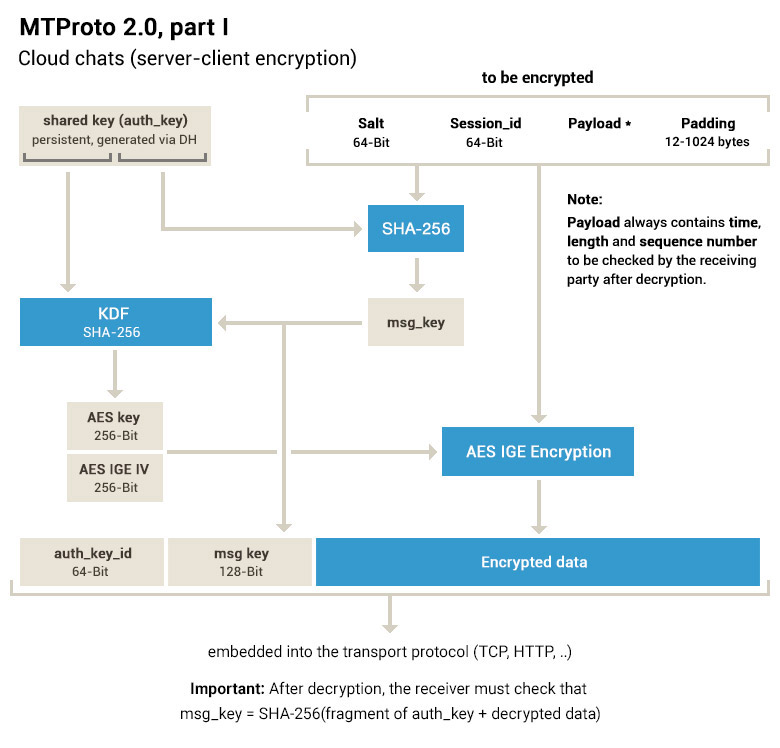
\includegraphics[scale=0.4]{imagenes/diagramaMTProto.jpg} 

\subsection{Resumen de los componentes}
\begin{description}
	\item \textbf{Componentes de alto nivel(Lenguajes de consulta/API RPC):}
Desde el punto de vista del componente de alto nivel, el cliente y el servidor intercambian mensajes dentro de una sesión.\\
La sesión se adjunta al cliente en lugar de una conexión \emph{websocket/http/https/tcp.} 
Además, cada sesión tiene asociada a clave ID de usuario mediante la cual se logra la autorización.\\ 
Pueden estar abiertas varias conexiones a un servidor, los mensajes pueden ser enviados en cualquier dirección a través de cualquiera de las conexiones.
Cuando se usa el protocolo UDP, una respuesta puede ser devuelta por una dirección de IP distinta.\\
Hay diferentes tipos de mensajes:
\begin{itemize}
		\item \textbf{LLamadas RPC(cliente-servidor):} LLamadas a los métodos de la API.
		\item \textbf{Respuestas RPC(servidor-cliente):} Resultados de las llamadas RPC.
		\item \textbf{Notificación del estado de los mensajes}
		\item \textbf{Consultas de estado de mensaje}
		\item \textbf{Mensaje multiparte o contenedor}
\end{itemize}
Desde el punto de vista de protocolos de bajo nivel, un mensaje es un flujo de datos alineados con 4 o 16 bytes de límite.
Los primeros campos en un mensaje están fijos y son usados por el sistema criptográfico o de autorización.\\
Cada mensaje, consiste en un \emph{Message Identifier} de 64 bits, \emph{número de secuencia del mensaje dentro de una sesión}, \emph{longitud} de 32 bits y \emph{cuerpo del mensaje} de cualquier tamaño siempre y cuando sea múltiplo de 4. 
Además cuando un contenedor o un mensaje simple se envían, una \emph{cabecera interna} se añade al principio del mensaje, luego el mensaje es cifrado y se le añade una \emph{cabecera externa} la cual será una \emph{clave de identificación} de 64 bits y una \emph{clave del mensaje} de 128 bits.\\
El \emph{cuerpo} del mensaje normalmente consiste en un \emph{tipo mensaje} de 32 bits seguido de los \emph{parámetros dependientes del tipo}.\\
Los números están escritos en \emph{little endian}. Sin embargo los números muy grandes(2048 bits) usados en \textbf{RSA} y \textbf{DH} están escritos en \emph{big endian} porque es lo que hace la biblioteca \textbf{OpenSSL}.
	\item \textbf{Autorización y Cifrado:}
			Antes de que un mensaje sea transmitido por la red usando un protocolo de transporte, este es cifrado añadiendo una cabecera externa la cual es insertada al principio del mensaje y contiene:
	\begin{itemize}
		\item \emph{Key Identifier} de 64 bits
		\item \emph{Message Key} de 128 bits
	\end{itemize}
Una clave de usuario junto con una clave de mensaje definen una clave de 256 bits la cual es la que cifra el mensaje usando un cifrado \emph{AES-256}.
La primera parte del mensaje cifrado contiene datos variables(sesión, id del mensaje, número de secuencia) los cuales influyen en la clave del mensaje. La clave del mensaje es definida como los 128 bits iniciales del mensaje cifrado con \emph{SHA-256}, 
además los mensajes en varias partes están cifrados como un solo mensaje.\\
Lo primero que tiene que hacer la aplicación cliente es crear una clave de autorización que se genera normalmente la primera vez que se ejecuta la aplicación y por lo general nunca cambia.\\
Para prevenir potenciales ataques debido a la apropiación de la clave de autorización MTProto soporta \emph{Perfect Forward Secrecy} tanto en los chats en la nube como en los chats secretos.
	\item \textbf{Sincronización de la hora:}
Si la hora de un cliente difiere de la hora del servidor, el servidor podría empezar a ignorar los mensajes de este y recíprocamente el cliente a los mensajes del servidor debido a que el mensaje tenga un indentificador inválido del mensaje.\\
Bajo estas circunstancias, el servidor enviará un mensaje especial al cliente el cual contendrá la hora correcta, este mensaje será el primero en el caso de que también se envíe un grupo de mensajes.\\
Habiendo recibido el mensaje, el cliente primero ejecutará una sincronización de la hora y después verificará la \emph{Message Key} para ver si es correcto.\\
En caso de que no sea correcto, el cliente deberá generar una nueva sesión para asegurar la monotonía de los \emph{Message Keys}.
\end{description}

\subsection{Descripción de las claves:}
En esta sección se describirán las distintas claves que entran en juego en el proceso de cifrado y descifrado de MTProto 2.0 \cite{telegram2}.

\begin{description}
	\item \textbf{Authorization Key (auth\textunderscore key)}\\
	Es una clave de 2048 bit compartida por el dispositivo del cliente y el servidor, se crea durante el registro del usuario, se almacena en el dispositivo de este mediante el protocolo de intercambio de claves \emph{Diffie-Hellman} y nunca se transmite a través de la red. Cada \emph{Authorization key} es única y dependiente del usuario, aunque un usuario puede tener más de una ya que Telegram permite tener sesiones persistentes en diferentes dispositivos. En caso de ser necesario estas claves pueden ser bloqueadas para siempre como por ejemplo podría pasar si un dispositivo con sesión persistente se pierde.

	\item \textbf{Server Key}\\
	Es una clave RSA de 2048 bits usada por el servidor para firmar sus mensajes durante el proceso de registro y la clave se está generando. La aplicación tiene una clave publica del servidor que puede ser utilizada para verificar la firmas pero no para firmar mensajes. La clave privada del servidor es almacenada en este y raramente cambia.

	\item \textbf{Key Identifier (auth\textunderscore key\textunderscore id)}\\
	Se usan los 64 bits menos significativos del hash \emph{SHA1} de la \emph{Authorization Key} para indicar que clave en particular se ha usado para cifrar el mensaje. Las claves tienen que ser identificadas unívocamente y en caso de colisión, la \emph{Authorization Key} se regenera. Un identificador Zero Key significa que el cifrado no se usa y esto está permitido para muy pocos mensajes usados durante el registro para generar la clave en el intercambio \emph{Diffie-Hellman}.
	
	\item \textbf{Session}\\
	Es un número de 64 bits generado aleatoriamente por el cliente para distinguir entre sesiones individuales como pueden ser diferentes instancias de la aplicación creadas con la misma \emph{Authorization Key} donde una instancia de la aplicación es la conjunción de la \emph{Key Identifier} y la \emph{Session}.\\
	Bajo ninguna circunstancia un mensaje perteneciente a una sesión puede ser enviado a otra.

	\item  \textbf{Server Salt}\\
	Es un número de 64 bits generado aleatoriamente que cambia cada 30 minutos independiente de las sesiones por una petición del servidor. Una vez generado el nuevo salt todos los mensajes tienen que tenerlo aunque se aceptan los mensajes con el salt previo. Es necesario para proteger ante ciertos ataques como podría ser ajustar el reloj de la víctima en un momento futuro.

	\item \textbf{Message Identifier (msg\textunderscore id)}\\
	Es un número de 64 bits dependiente del tiempo usado únicamente para identificar mensajes sin sesión. Los \emph{Message Identifiers} son divisibles por 4, los \emph{Message Identifiers} del servidor módulo 4 dan 1 si el mensaje es una respuesta a un mensaje del cliente y dan 3 en otro caso. 
	Los \emph{Message Identifiers} del cliente deben incrementarse monótonamente, igualmente con los del servidor y tienen que ser aproximadamente igual a $unixtime*2^{32}$, donde \emph{unixtime} es un sistema para la descripción de instantes de tiempo definida como la cantidad de segundos transcurridos desde la medianoche UTC del 1 de enero de 1970. 
	De esta manera, el \emph{Message Identifier} señala el momento aproximado en el que el mensaje fue creado siendo rechazado alrededor de 300 segundos después o 30 segundos antes de ser creado (necesario como medida de protección de ataques de repetición).  

	\item \textbf{Content-related Message}\\
	Un mensaje requiere un reconocimiento explícito. Esto incluye todos los mensajes de usuario y muchos de servicio, a excepción de contenedores y otros reconocimientos.

	\item \textbf{Message Sequence Number (msg\textunderscore seqno)}\\
	Un número de 32 bit igual o el doble del número de mensajes \emph{content-related} creados por el remitente antes de este mensaje y posteriormente se va incrementado en uno si el mensaje es del tipo \emph{cotent-related}. Cabe a destacar que como un contenedor se genera después de su contenido, su \emph{Message Sequence Number} será siempre igual o mayor a los números de mensajes contenidos en él.

	\item \textbf{Message Key (msg\textunderscore key)}\\
	En el protocolo \textbf{MTProto 2.0}, la \emph{Message Key} se define como los 128 bits del medio del hash \emph{SHA-256} del mensaje que va a ser cifrado antepuesto por un fragmento de 32 bytes de la clave de autorización.\\
	En el protocolo \textbf{MTProto 1.0}, la \emph{Message Key} se definía como los 128 bits menos significativos del hash \emph{SHA-1} del mensaje a ser cifrado, los bytes de relleno eran excluidos en el cálculo del hash. La \emph{Authorization Key} no estaba involucrada en este cálculo.

	\item \textbf{Internal (cryptographic) Header}\\
	Una cabecera de 16 bytes añadida antes de que el mensaje o el contenedor sea cifrado. Consiste en el \emph{Server Salt} de 64 bits y la \emph{Session} de 64 bits.

	\item \textbf{External (cryptographic) Header}\\
	Una cabecera de 24 bytes que se añade antes de que el mensaje o el contenedor sea cifrado. Consiste en la \emph{auth\textunderscore key\textunderscore id} de 64 bits y la \emph{msg\textunderscore key} de 128 bits.

	\item \textbf{Payload}\\
	Es el \emph{External Header} + mensaje cifrado o contenedor.
\end{description}

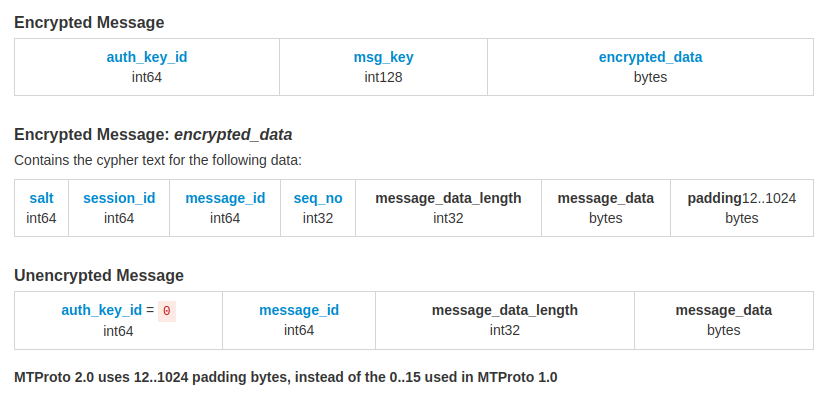
\includegraphics[scale=0.5]{imagenes/MTProto2.png} 

\subsection{Creación de la \emph{Authorization Key}}
Como hemos visto en el apartado anterior la \emph{Authorization Key} se genera durante el registro del usuario en la aplicación. El formato de las consultas usa \emph{Binary Data Serialization} ya que MTProto requiere que los tipos de datos estén en formato binario y \emph{TL Language} que sirve para describir el sistema utilizado de tipos y funciones.\\
Los números de gran tamaño son transmitidos como cadenas que contienen la secuencias de bytes en formato \emph{big endian}, los números de menor tamaño como pueden ser los \emph{int, long int128...} usan normalmente el formato \emph{little endian} aunque si pertenecen al \emph{SHA1} los bytes no son reorganizado.\\
Una vez introducido los formatos que seguirán las consultas y los números veamos los pasos que se siguen en la creación de la \emph{Authorization Key}.

\begin{enumerate}
	\item El cliente envía una consulta al servidor, en esta consulta irá el \emph{nonce} que es un número aleatorio \emph{int128} generado por el cliente que servirá para para que el servidor lo identifique, este número no es secreto y a partir de ese momento irá incorporado en todas las consultas. 
	
	\item El servidor le responde enviándole: 
	\begin{itemize}
		\item \emph{server\textunderscore nonce}: Es un número aleatorio \emph{int128} generado por el servidor que sirve para que el cliente lo identifique y al igual que el \emph{nonce} no será secreto e irá incluido en las siguientes consultas y respuestas. 
		\item \emph{pq}: Es una representación de un número natural en formato \emph{big endian} que es el producto de dos números primos, \emph{pq} por lo general verifica $pq \leq 2^{63}-1$
		\item \emph{server\textunderscore public\textunderscore key\textunderscore fingerprints}: Es una lista de \emph{fingerprints} de claves RSA públicas.
	\end{itemize}

	\item El cliente descompone \emph{pq} en factores primos tal que $p$\textless$q$. Con esto empieza el intercambio de claves Diffie-Hellman.

	\item El cliente envía una nueva consulta que contiene:
	\begin{itemize}
		\item \emph{nonce}
		\item \emph{server\textunderscore nonce}
		\item \emph{p}: Factor obtenido en el paso anterior, es de tipo \emph{long}.
		\item \emph{q}: El otro factor obtenido en el paso anterior, al igual que \emph{p} es de tipo \emph{long}.
		\item \emph{public\textunderscore key\textunderscore fingerprint}: Una de las \emph{fingerprints} obtenida de la lista enviada por el servidor en el paso anterior, es del tipo \emph{long}.
		\item \emph{encrypted\textunderscore data}: Mensaje cifrado obtenido aplicando RSA a \emph{data} y \emph{server\textunderscore public \textunderscore key} donde:
		\begin{itemize}
			\item \emph{data}: Es una serialización de \emph{pq}, \emph{p}, \emph{q}, \emph{nonce}, \emph{server\textunderscore nonce}, \emph{new\textunderscore nonce} (un nuevo número aleatorio generado por el cliente y desde este paso conocido por el cliente y el servidor) y \emph{dc} o una serialización de \emph{pq}, \emph{p}, \emph{q}, \emph{nonce}, \emph{server\textunderscore nonce}, \emph{new\textunderscore nonce}, \emph{dc} y \emph{expires\textunderscore in}.

			\item \emph{dc} es un identificador de la consulta, es del tipo \emph{int}.

			\item \emph{expires\textunderscore in} es el tiempo en el que expira la consulta, es del tipo \emph{int}.
		\end{itemize}
	\end{itemize}
	Después de este paso alguien podría interceptar la consulta y modificarla con una cosulta suya haciendo un ataque \textbf{man-in-the-middle}. 
	Este ataque no sería muy efectivo, ya que el único elemento que podría modificar sería \emph{new\textunderscore nonce} porque los demás están cifrados y el resultado sería que el atacante genere una \emph{Authorization\textunderscore key} propia independiente de la del cliente haciendo que el ataque no sea efectivo.

	\item El servidor responde enviando:
		\begin{itemize}
			\item \emph{nonce}
			\item \emph{server\textunderscore nonce}
			\item \emph{encrypted\textunderscore answer}: Respuesta cifrada que es del tipo \emph{string} y contiene:
			\begin{itemize}
				\item \emph{new\textunderscore nonce\textunderscore hash}: Son los 128 bits menos significativos de \emph{SHA1(new\textunderscore nonce)}.
				\item \emph{answer}: Es una serialización de \emph{nonce}, \emph{server\textunderscore nonce}, \emph{g}, \emph{dh\textunderscore prime}, \emph{g\textunderscore a} y \emph{server\textunderscore time}.
				\item \emph{answer\textunderscore with\textunderscore hash}: Es una generación con la función hash \emph{HASH1} quedando de la siguiente forma: \emph{SHA1(answer)+answer+(0-15 bytes aleatorios)} de manera que la longitud sea divisible por 16, es del tipo \emph{string}.
				\item \empph{answer\textunderscore aes\textunderscore key}: \emph{SHA1(new\textunderscore nonce + server\textunderscore nonce) + substr(SHA1(server\textunderscore nonce + new\textunderscore nonce), 0, 12)} y es del tipo \emph{string}.
				\item \emph{tmp\textunderscore aes\textunderscore iv}: \emph{substr(SHA1(server\textunderscore nonce + new\textunderscore nonce), 12, 8) + SHA1(new\textunderscore nonce + new\textunderscore nonce) + substr(new\textunderscore, 0, 4)}
				\item \emph{encrypted\textunderscore answer}: \emph{AES256\textunderscore ige\textunderscore encrypt(answer\textunderscore with\textunderscore hash, tmp\textunderscore aes\textunderscore key, tmp\textunderscore aes\textunderscore iv)} donde:
				\begin{itemize}
					\item \emph{tmp\textunderscore aes\textunderscore key}: Es una clave de 256 bits
					\item \emph{tmp\textunderscore aes\textunderscore iv}: Es un vector de inicialización de 256 bits.
				\end{itemize}
				Al igual que en el resto de las instancias que usan el cifrado AES, a los datos cifrados se le añaden bytes aleatorios de forma que el tamaño sea divisible por 16.
			\end{itemize}
		\end{itemize}
	Después de este paso \emph{new\textunderscore nonce} sigue siendo únicamente conocido por el cliente y el servidor de esta manera el cliente garantiza que el servidor es el que está al otro lado de la comunicación y que la respuesta de este es correcta, ya que los datos están cifrados usando \emph{new\textunderscore nonce}.\\
	El cliente comprueba que \emph{p} el cual es un primo usado en Diffie-Hellman, es un número primo seguro de 2048 bits, es decir, se tiene que verificar que \emph{p} y $\frac{p-1}{2}$ son primos, además, $2^{2047}$\textless \emph{p} \textless $2^{2048}$, y \emph{g} genera un subgrupo cíclico con orden primo $\frac{p-1}{2}$.\\
	Si la verificación tarda mucho tiempo, cosa que ocurre en dispositivos antiguos, se ejecutarían solo 15 iteraciones en el algoritmo de Miller-Rabin para garantizar que \emph{p} y $\frac{p-1}{2}$ sean primos con una probabilidad de error muy baja, alrededor de una millonésima, y dejar el resto de iteraciones para después, ejecutándose estas de fondo.

	\item El cliente genera un número aleatorio \emph{b} de 2048 bits y lo envía al servidor en un mensaje que contiene:
		\begin{itemize}
			\item \emph{nonce}
			\item \emph{server\textunderscore nonce}
			\item \emph{encrypted\textunderscore data} que se descifra de la siguiente manera:
				\begin{itemize}
					\item \emph{g\textunderscore b} = $g^b$ mod \emph{dh\textunderscore prime}
					\item \emph{data} que es una serialización donde:
						\begin{itemize}
							\item \emph{nonce}
							\item \emph{server\textunderscore nonce}
							\item \emph{retry\textunderscore id} que vale 0 en el primer intento y en caso contrario, vale \emph{auth\textunderscore key\textunderscore aux\textunderscore hash} del intento fallido anterior y es del tipo \emph{long}.
							\item \emph{g\textunderscore b} que es del tipo \emph{string}.
						\end{itemize}
					\item \emph{data\textunderscore with\textunderscore hash} que es: \emph{SHA1(data)+data+(0-15 bytes aleatorios de manera que el tamaño sea divisible por 16)}.
					\item \emph{encrypted\textunderscore data} que es: \emph{AES256\textunderscore ige\textunderscore encrypt(data\textunderscore with\textunderscore hash, tmp\textunderscore aes\textunderscore key, tmp\textunderscore aes\textunderscore iv)}.
				\end{itemize}
		\end{itemize}
	\item Una vez hecho los pasos previos tendríamos que \emph{auth\textunderscore key} vale $g^{ab}$ mod \emph{dh\textunderscore prime}, en el servidor se calcula como \emph{$g\textunderscore b^{a}$ mod \emph{dh\textunderscore prime}} y en el cliente se calcula como $g\textunderscore a^b$ mod \emph{dh\textunderscore prime}.
	\item \emph{auth\textunderscore key\textunderscore hash} se calcula como los 64 bits de menor prioridad de \emph{SHA1(auth\textunderscore key)}. El servidor comprueba si existe alguna otra clave con el mismo \emph{auth\textunderscore hash} y responde de alguna de las siguientes tres formas
	\begin{enumerate}
		\item Una serialización de: 
			\begin{itemize}
				\item \emph{nonce}
				\item \emph{server\textunderscore nonce}
				\item \emph{new\textunderscore nonce\textunderscore hash1}
			\end{itemize}
		\item Una serialización de:
			\begin{itemize}
				\item \emph{nonce}	
				\item \emph{server\textunderscore nonce}
				\item \emph{new\textunderscore nonce\textunderscore hash2}
			\end{itemize}
		\item Una serialización de:
			\begin{itemize}
				\item \emph{nonce}	
				\item \emph{server\textunderscore nonce}
				\item \emph{new\textunderscore nonce\textunderscore hash3}
			\end{itemize}
	\end{enumerate}
	Donde \emph{new\textunderscore nonce\textunderscore hash1}, \emph{new\textunderscore nonce\textunderscore hash2} y \emph{new\textunderscore nonce\textunderscore hash3} son los 128 bits menos significativos de SHA1 de la cadena de bytes obtenida al añadir a \emph{new\textunderscore nonce} un byte con el valor 1,2 o 3 respectivamente y seguido de \emph{auth\textunderscore key\textunderscore hash}.\\
	\emph{Auth\textunderscore key\textunderscore aux\textunderscore hash} son los 64 bits más significativos de \emph{SHA1(auth\textunderscore key)}.
	Si algo falla durante estos pasos, el cliente volvería al paso 6 y generándose un nuevo \emph{b}. Al mismo tiempo se define \emph{server\textunderscore salt} como \emph{substr(new\textunderscore nonce, 0, 8)} XOR \emph{substr(server\textunderscore nonce, 0, 8)}.\\
	
\end{enumerate}
\textbf{Gestión de errores}

Si el cliente no obtiene alguna respuesta del servidor en un intervalo de tiempo determinado se repite la consulta, análogamente ocurre con el servidor. Sin embargo si el servidor no obtiene una segunda respuesta del cliente en 10 minutos, reiniciará la conexión y el cliente tendrá que empezar de nuevo.

\subsection{Generando la clave y el vector de inicialización de AES}
En esta sección hablaré de como se generan la clave de autorización (\emph{auth\textunderscore key}) y de la clave del mensaje (\emph{msg\textunderscore key}) necesarias para calcular la clave de AES (\emph{aes\textunderscore key}) y el vector de inicialización de 256 bits (\emph{iv\textunderscore aes}) usados para cifrar los mensajes en MTProto 2.0.\\
El algoritmo consiste en:
\begin{enumerate}
	\item Calculamos \emph{msg\textunderscore key\textunderscore large} como \emph{SHA256(substr(auth\textunderscore 88+x, 32)+plaintext+random\textunderscore padding)}.
	\item Calculamos \emph{msg\textunderscore key} como \emph{substr(msg\textunderscore key\textunderscore large, 8, 16)}.
	\item Calculamos \emph{sha256\textunderscore a} como \emph{SHA256(msg\textunderscore key+substr(auth\textunderscore key, x, 36))}.
	\item Calculamos \emph{sha256\textunderscore b} como \emph{SHA256(substr(auth\textunderscore key, 40+x, 36)+msg\textunderscore key)}
\end{enumerate}
Y una vez hechos estos pasos, ya podemos calcular la clave para AES y el vector de inicialización.
\begin{itemize}
	\item \textbf{\emph{aes\textunderscore key}}: \emph{substr(sha256\textunderscore a, 0, 8)+substr(sha256\textunderscore b, 8, 16)+substr(sha256\textunderscore a, 24, 8)}.
	\item \textbf{\emph{aes\textunderscore iv}}: \emph{substr(sha256\textunderscore b, 0, 8) + substr(sha256\textunderscore a, 8 16)+substr(sha256\textunderscore b, 24, 8)}.
\end{itemize}
\emph{x} vale 0 cuando los mensajes van del cliente al servidor y 8 cuando los mensajes van del servidor al cliente.\\
Los 1024 bits menos significativos de la \emph{auth\textunderscore key} no se utilizan para el cálculo ya que estos se usan para cifrar la copia local de los datos recibidos del servidor además, los 512 bits menos significativos no se almacenan en el servidor por lo que si el cliente pierde la clave o la contraseña del dispositivo, no se podrán descifrar los datos locales.
